\section{Theorie}
\label{sec:Theorie}

% In knapper Form sind die physikalischen Grundlagen des Versuches, des Messverfahrens, sowie sämtliche für die Auswertung erforderlichen Gleichungen darzustellen. (Keine Herleitung)

% (eventuell die Aufgaben)

% Der Versuchsaufbau: Beschreibung des Versuchs und der Funktionsweise (mit Skizze/Bild/Foto)

\subsection{Aufbau des Franck-Hertz-Versuchs}
\label{ssec:aufbau}

Eine Möglichkeit die diskreten Energieniveaus eines Atoms zu zeigen sind Elektronenstoßexperimente, wie der Franck-Hertz-Versuch.
Die grundliegende Idee ist dabei, die Atome mit energetischen Elektronen zu beschießen und den Energieverlust zu bebachten. 
Es treten elastische und unelastische Stöße auf.
Dabei wird bei einem unelastischen Stoß exakt die Energie benötigt, die das Atom braucht um von seinem Grundzustand in einen angeregten Zustand überzugehen, also 
\begin{equation}
    E_1 - E_0 = \frac{m_0 \cdot v^2_\text{vor}}{2} - \frac{m_0 \cdot v^2_\text{nach}}{2}.
    \label{eq:energiedif}
\end{equation}
Im Folgenden wird versucht diese Energiediffernz zu bestimmen.
Dafür wird eine Versuchsapperatur nach \autoref{fig:aufbau} verwendet.

\begin{figure}
    \centering
    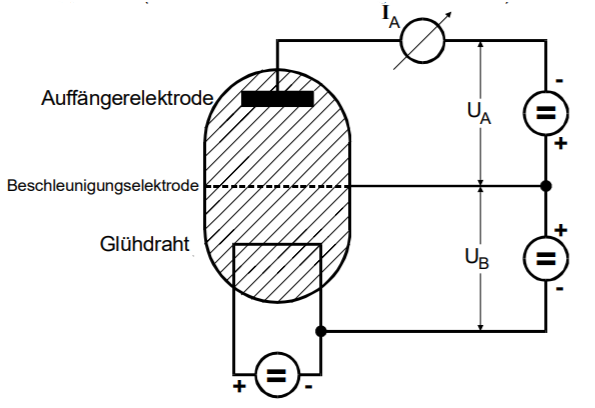
\includegraphics[width=0.6\textwidth]{images/bild1.png}
    \caption{Schematischer Aufbau des Franck-Hertz-Versuchs.\cite{V601}}
    \label{fig:aufbau}
\end{figure}

In einem evakuierten Gefäß wird Quecksilber zum Verdampfen gebracht, daraufhin entsteht ein Sättigungsdampfdruck $p_\text{sät}$, der über eine Temperatur $T$ gesteuert werden kann.
Es wird eine Glühkathode aus Wolfram auf Rotglut erhitzt, diese emittiert dann Elektronen.
Die Elektronen bewegen sich zur Beschleunigungselektrode hin, an der die Beschleunigungsspannung $U_\text{B}$ anliegt. 
Der Abstand zwischen Elektrode und Glühkathode ist die Beschleunigunsstrecke, passieren die Elektronen diese Strecke haben sie die Energie
\begin{equation}
    \frac{m_0 \cdot v^2_\text{vor}}{2} = e_0 \cdot U_\text{B},
    \label{eq:beschleu}
\end{equation}
wenn zu Beginn die Geschwindigkeit 0 angenommen wird.
Der letzte Teil des Gefäßes ist die Auffängerelektrode, an diese ist die Abbremsspannung $U_\text{A}$ angelegt.
Alle Elektronen müssen diese Barriere überwinden, um zur Elektrode zur gelangen und detektiert zu werden, geschieht das kann ein Strom $I_\text{A}$ gemessen werden.

\subsection{Funktionsweise des Franck-Hertz-Versuchs}
\label{ssec:funktion}

Auf der Beschleunigunsstrecke kommt es zwangsweise zu Zusammenstößen zwischen Elektronen und Hg-Atomen, diese können wie schon beschrieben elastisch oder unelastisch sein.
Bei einem Elastischen, war die Elektronenenergie nicht hoch genug das Atom anzuregen und es wird weggeschlagen.
Nur, wenn die Energie hoch genug ist, kann das Atom angeregt werden.
Das Hg-Atom bleibt nicht in diesen Zustand, sondern sendet ein Lichtquant mit der Energie
\begin{equation}
    \nu \cdot h = E_1 - E_0
    \label{eq:quant}
\end{equation}
aus, Dabei ist $\nu$ die Frequenz und $h$ das Plancksche Wirkungsquantum.
Danach ist das Atom wieder in seinem Grundzustand und kann erneut angeregt werden.
Wird der Auffängerstrom $I_\text{A}$ gegen die Beschleunigungsspannung $U_\text{B}$ aufgetragen entsteht eine Abbildung wie in \autoref{fig:kurve}.

\begin{figure}
    \centering
    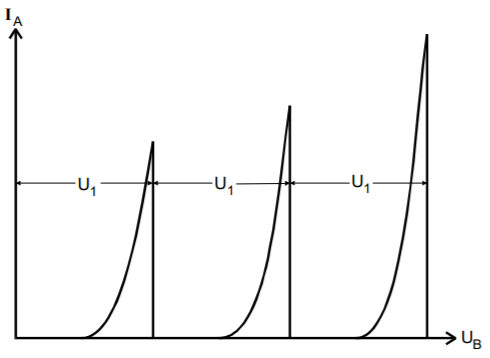
\includegraphics[width=0.6\textwidth]{images/bild2.png}
    \caption{Theoretisches Ergebnis des Franck-Hertz-Versuchs.\cite{V601}}
    \label{fig:kurve}
\end{figure}

Zu Beginn ist der Zusammenhang trivial, wird $U_\text{B}$ erhöht, sind mehr Elektronen energetisch genug um die Bremsspannung zu überwinden.
Im weiteren Verlauf bricht die Kurve ein und fällt auf null, dies geschieht, weil die Elektronen die nötige Energie erreicht haben die Hg-Atome anzuregen.
Durch den Energieverlust aus \eqref{eq:energiedif} haben die Elektronen nach dem Zusammenstoß nicht mehr genug Energie um die Auffängerelektrode zu erreichen. 
Wird die Beschleunigungsspannung noch weiter erhöht besitzten sie wieder genug Energie, allerdings wird die Kurve erneut einbrechen, da sie bei genügend Beschleunigiung sogar zwei mal ein Atom anregen können.
Der Abstand der Maxima $U_1$ kann dann über 
\begin{equation}
    U_1 = \frac{1}{e_0}(E_1 - E_0)
    \label{eq:quant}
\end{equation}
berechnet werden.

\subsection{Einflüsse auf die Franck-Hertz-Kurve}
\label{ssec:einfluss}

Die tatsächliche Beschleunigung der Elektronen ist nicht durch $U_\text{B}$ gegeben, sondern leicht verschieden.
Aufgrund der Tatsache, dass die beiden Elektroden verschiedene Austrittsarbeiten besitzen und sich berühren werden Elektronen umherwandern.
Dieses Phänomen wird Kontaktpotenital genannt und ist in \autoref{fig:kontakt} graphisch dargestellt.

\begin{figure}
    \centering
    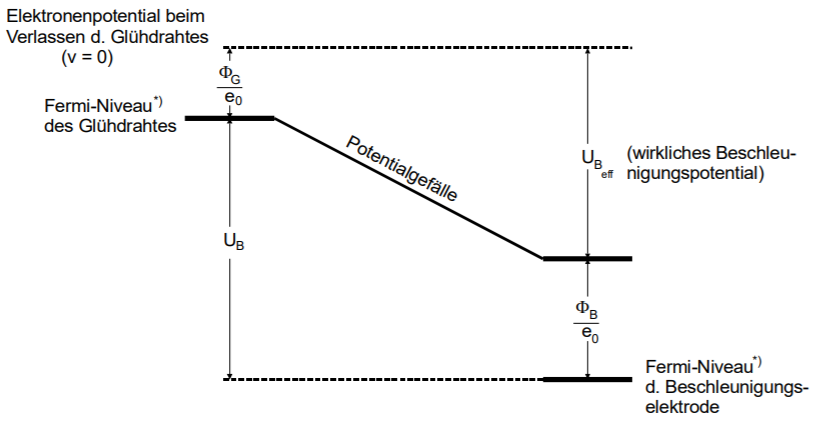
\includegraphics[width=0.6\textwidth]{images/bild3.png}
    \caption{Tatsächliches Potentialverhältnis zwischen den Elektroden.\cite{V601}}
    \label{fig:kontank}
\end{figure}

Daraus ergibt sich das tatsächliche Beschleunigungspotential 
\begin{equation}
    U_\text{B,eff} = U_\text{B} - \frac{1}{e_0} \left(\Phi_\text{B} - \Phi_\text{G} \right)
    \label{eq:ueff}
\end{equation}
mit dem sogenannten Kontaktpotenital K
\begin{equation}
    K = \frac{1}{e_0} \left(\Phi_\text{B} - \Phi_\text{G} \right).
    \label{eq:kontakt}
\end{equation}
Die Franck-Hertz-Kurve ist um den Wert $K$ verschoben.

Einen weiteren Einfluss hat die Energieverteilung der Elektronen, diese ist nämlich nicht konstant, sondern in einem Energiespektrum verteilt. 
Das bedeutet manche Elektronen sind früher in der Lage unelastische Stöße durchzuführen als andere.
Für die Kurve bedeutet das, dass sie nach Beginn des Experimentes nie mehr ganz auf null fallen wird und leicht verformt wird.
Daher ist es wichtig dieses Spektrum zu kennen, bevor der eigentliche Versuch durchgeführt wird.
Es kann ebenfalls einen Effekt haben, wenn die Elektronen, die zum Auffängerstrom beitragen würden durch elastische Stöße weggestoßen werden. Das führt zu einem Abflachen der Kurve.

Eine weitere wichtige Größe ist die mittlere freie Weglänge $\bar{w}$. 
Sie muss klein gegen die Beschleunigunsstrecke sein, damit es zu möglichst vielen Zusammenstößen kommt.
Dabei hängt sie mit dem Sättigungsdampfdruck zusammen, und damit auch mit der Temperatur $T$.
Die mittlere freie Weglänge lässt sich über 
\begin{equation}
    \bar{w} = \frac{0.0029}{p_\text{sät}}
    \label{eq:wegl}
\end{equation}
bestimmen.
Hier ist die Weglänge in $\si{\centi\meter}$ und $p_\text{sät}$ in $\si{\milli\bar}$ angegeben.
Der Sättigungsdampfdruck ist als 
\begin{equation}
    p_\text{sät} = 5.5 \cdot 10^7 \cdot \exp{\left(\frac{-6876}{T}\right)}
    \label{eq:dampfdr}
\end{equation}
definiert.
